\begin{exercice}
Calcule le périmètre et l'aire de la plaque métallique représentée ci‑dessous :
\begin{center} 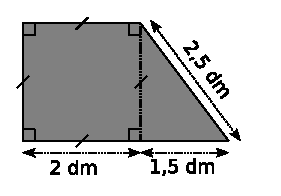
\includegraphics[width=3.6cm]{plaque} \end{center}
\end{exercice}


\begin{exercice}
La figure suivante représente un morceau de tissu. Calcule son aire :
\begin{center} 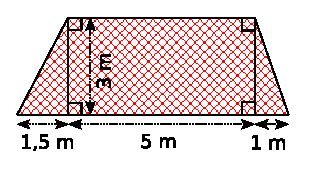
\includegraphics[width=4.4cm]{tissu} \end{center}
\end{exercice}


\begin{exercice}
On souhaite entourer, avec du grillage, un jardin carré de 24 m de côté, en laissant une ouverture de 4 m de large. Le grillage choisi coûte 15 CHF le mètre. Quel sera le prix à payer ?
\end{exercice}


\begin{exercice}
M. Albert vend un terrain représenté ci‑dessous au prix de 18 CHF le m\up{2} :
\begin{center} 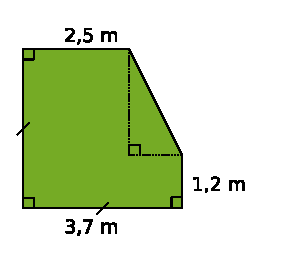
\includegraphics[width=3.7cm]{Albert} \end{center}
Quel est le prix de vente de ce terrain ?
\end{exercice}


\begin{exercice}
Dans une pièce de bois rectangulaire de dimensions 10,2 cm sur 6,6 cm, un menuisier découpe un losange dont les sommets se trouvent au milieu de chaque côté du rectangle :
\begin{center} 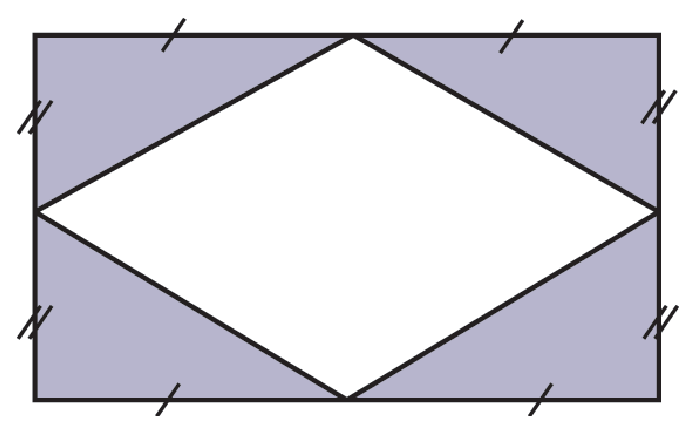
\includegraphics[width=4.6cm]{losange_bois} \end{center}
Calcule l'aire du losange.
\end{exercice}


\begin{exercice}
Sur le mur d’une salle de bains, on a posé 10 rangées de 14 carreaux de 12 cm de côté. Quelle est, en m\up{2}, l’aire de la surface carrelée ?
\end{exercice}


\begin{exercice}
Un rectangle a pour longueur 12,3 dm et pour largeur 48,5 cm :
\begin{enumerate}
 \item Calcule le périmètre de ce rectangle en cm puis en dm ;
 \item Calcule l'aire de ce rectangle en cm\up{2} puis en dm\up{2}.
 \end{enumerate}
\end{exercice}


\begin{exercice}[Agrandissement]
Un rectangle a pour dimensions 4,3 m et 7,8 m :
\begin{enumerate}
 \item Calcule son périmètre et son aire ;
 \item On double sa largeur et sa longueur.
 
Calcule de nouveau son périmètre et son aire ;
 \item Que constates-tu ?
 \end{enumerate}
\end{exercice}


\begin{exercice}[Même aire]
Construis un carré, un rectangle (non carré) et un triangle rectangle ayant chacun pour aire 16 cm\up{2}.
\end{exercice}


\begin{exercice}[Du rectangle au carré]
\begin{enumerate}
 \item Construis un rectangle de dimensions 5,1 cm et 3,3 cm ;
 \item Construis un carré ayant le même périmètre que ce rectangle ;
 \item Le rectangle et le carré ont-ils la même aire ? Explique.
 \end{enumerate}
\end{exercice}


\begin{exercice}
On considère la figure suivante :
\begin{center} 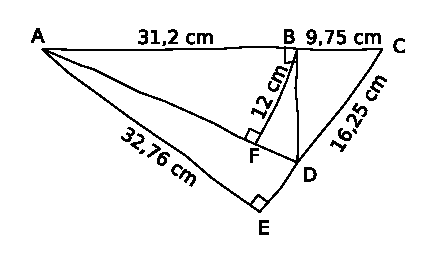
\includegraphics[width=6cm]{croquis_grand} \end{center}
\begin{enumerate}
 \item Quelle est la hauteur relative au côté $[CD]$ pour le triangle $ACD$ ?
 \item Calcule l'aire du triangle $ACD$ et la longueur $[BD]$.
 \item Calcule $[AD]$.
 \end{enumerate}
\end{exercice}


\begin{exercice}[Des rectangles]
Les rectangles $R_1$, $R_2$, $R_3$, $R_4$ et $R_5$ ont tous un périmètre de 20 cm mais des tailles différentes.

\begin{center}
\begin{tabularx}{\linewidth}{|c|*{6}{>{\centering \arraybackslash}X|}}
\hline  & \cellcolor{A1} $R_1$ & \cellcolor{A1} $R_2$ & \cellcolor{A1} $R_3$ & \cellcolor{A1} $R_4$ & \cellcolor{A1} $R_5$ \\
\hline \cellcolor{H1} Longueur d'un côté (en cm) & 1 & 2 & 3 & 4 & 5 \\
\hline \cellcolor{H1} Longueur de l'autre côté (en cm) & & & & & \\
\hline \cellcolor{H1} Aire (en cm\up{2}) & & & & & \\
\hline
\end{tabularx} \\
\end{center}

\begin{enumerate}
 \item Reproduis et complète le tableau ci-dessus.
 \item Construis chacun de ces rectangles.
 
Y en a‑t‑il un particulier ? Lequel et pourquoi ?
 \item Dans un tableur, reproduis un tableau similaire à celui‑ci. Fais effectuer les calculs jusqu'au rectangle $R_9$ en allant de 0,5 cm en 0,5 cm pour la longueur d'un côté. Tu pourras afficher une représentation graphique de ce tableau. \\[0.5em]
Quel rectangle semble avoir la plus grande aire ?
 \end{enumerate}
\end{exercice}


\begin{exercice}[Quadrilatères inconnus]
Dans chaque cas, construis tous les quadrilatères qui satisfont aux énigmes suivantes :
\begin{enumerate}
 \item Je suis un rectangle. Mes côtés ont des mesures entières. Mon aire est de 18 cm\up{2} et mon périmètre est supérieur à 20 cm. 
 \item Je suis un quadrilatère dont les angles opposés sont égaux deux à deux. Mon aire vaut 24 cm\up{2} et mon périmètre 22 cm. Mes côtés ont des mesures entières.
 \item Je suis un quadrilatère non croisé qui a deux côtés consécutifs égaux et qui possède ses diagonales perpendiculaires. Mon aire vaut 24 cm\up{2}. Mes diagonales ont des mesures entières et se coupent au quart de la plus grande diagonale.
 \end{enumerate}
\end{exercice}


